\documentclass[t,14pt]{beamer}

\input setup.tex
\input macros.tex

\usepackage{multicol}

\date[Introduction]{Support Vector Machines}

%%%%%%%%%%%%%%%%%%%%%%%%%%%%%%%%%%%%%%%%%%%%%%%%%%%%%%%%%%%%%%%%%%%%%%
\begin{document}

\begin{frame}
  \titlepage
\end{frame}

%%%%%%%%%%%%%%%%%%%%%%%%%%%%%%%%%%%%%%%%%%%%%%%%%%%%%%%%%%%%%%%%%%%%%%
\section{Support Vector Machines}

%%%%%%%%%%%%%%%%%%%%%%%%%%%%%%%%%%%%%%%%%%%%%%%%%%%%%%%%%%%%%%%%%%%%%%
\subsection{SVMs for regression}

\begin{frame}
  \frametitle{Error function in regression}
  In simple regression, the objective is to minimize a regularized error 
  function
  \begin{equation}
    \frac{\displaystyle 1}{\displaystyle 2}
        \sum\limits_{n=1}^N \{y_n - t_n\}^2 + 
        \frac{\displaystyle \lambda}{\displaystyle 2}{\lVert w \rVert}^2
  \end{equation}

  To obtain sparse solutions, the above equation can be replaced by a 
  $\epsilon \textit{ - insensitive error function}$
  \begin{equation}
    E_\epsilon(y(\mathbf{x}) - t) = 
        \begin{cases}
            0 & \text{if } \lvert y(x) - t \rvert < \epsilon \\
            \lvert y(x) - t \rvert - \epsilon & \text{otherwise}
        \end{cases}
  \end{equation}
\end{frame}

\begin{frame}
  \frametitle{Minimizing the error function}
  To obtain the solution, minimize the regularized error function
  \begin{equation}
    C \sum\limits_{n=1}^N E_\epsilon(y(\mathbf{x}_n) - t_n) + 
      \frac{\displaystyle 1}{\displaystyle 2}{\lVert w \rVert}^2
  \end{equation} 
  where $C$ is the (inverse) regularization parameter
\end{frame}

\begin{frame}
  \frametitle{Error function with slack variables}
  By introducing slack variables for each data point $x_n$\\
  \begin{itemize}
    \item {$\xi_n \geq 0$ where $t_n > y(\mathbf{x}_n) + 
  \epsilon$} 
    \item {$\widehat{\xi}_n \geq 0$ where $t_n < y(\mathbf{x}n) 
  + \epsilon$} 
  \end{itemize}
  the error function can be written as
  \begin{equation}
    C \sum\limits_{n=1}^N (\xi_n + \widehat{\xi}_n) + 
        \frac{\displaystyle 1}{\displaystyle 2}{\lVert w \rVert}^2
  \end{equation}
  This is to be minimized subject to the constraints
  \begin{itemize}
    \item {$\widehat{\xi}_n \geq 0$ and $\xi \geq 0$}
    \item {$t_n \leq y(\mathbf{x}_n) + \epsilon + \xi_n$}
    \item {$t_n \geq y(\mathbf{x}_n) - \epsilon - \widehat{\xi}_n$}
  \end{itemize}
\end{frame}

\begin{frame}
  \frametitle{SVM Regression \textit{tube}}
  \includegraphics[trim=2cm 0cm 0cm 5cm,clip,scale=0.5,page=9]{Chapter_7.pdf}
\end{frame}

\begin{frame}
  \frametitle{Applying Lagrange multipliers}
  Plugging in the Lagrange multipliers and simplifying,
  \begin{align} 
    \widetilde{L}(\mathbf{a}, \widehat{\mathbf{a}}) &= 
        -\frac{\displaystyle 1}{\displaystyle 2}
        \sum\limits_{n=1}^N \sum\limits_{m=1}^N 
            (a_n - \widehat{a}_n)(a_m - \widehat{a}_m)
            k(\mathbf{x}_n,\mathbf{x}_m) \nonumber \\
            &\quad - \epsilon \sum\limits_{n=1}^N(a_n - \widehat{a}_n)
            + \sum\limits_{n=1}^N(a_n - \widehat{a}_n)t_n
  \end{align}
  where $a_n \geq 0$ and $\widehat{a_n} \geq 0$ are the Lagrange multipliers; 
  and\\
  $k(\mathbf{x}, \mathbf{x'}) = \phi(\mathbf{x})^T \phi(\mathbf{x'})$ is the 
  kernel.
\end{frame} 

\begin{frame}
  \frametitle{Predicting new inputs}
  The prediction can be made for new inputs using
  \begin{equation}
    y(\mathbf{x}) = \sum\limits_{n=1}^N (a_n - \widehat{a}_n)
                                        k(\mathbf{x}, \mathbf{x}_n)
                    + b
  \end{equation}
\end{frame}

%%%%%%%%%%%%%%%%%%%%%%%%%%%%%%%%%%%%%%%%%%%%%%%%%%%%%%%%%%%%%%%%%%%%%%
\subsection{$\nu$-SVMs}

\begin{frame}
  \frametitle{$\nu$-SVMs}
  \begin{itemize}
    \item {An alternative for of SVM for regression}
    \item {
            Use a parameter $\nu$ that bounds the fraction of points lying 
            \textit{outside} the tube instead of fixing the width $\epsilon$ 
            of the \textit{insensitive} region
          }
  \end{itemize}
\end{frame}

\begin{frame}
  \frametitle{Maximizing the dual}
  \vspace{-2em}
  \begin{align} 
    \widetilde{L}(\mathbf{a}, \widehat{\mathbf{a}}) &= 
        -\frac{\displaystyle 1}{\displaystyle 2}
        \sum\limits_{n=1}^N \sum\limits_{m=1}^N 
            (a_n - \widehat{a}_n)(a_m - \widehat{a}_m)
            k(\mathbf{x}_n,\mathbf{x}_m) \nonumber \\
            &\quad + \sum\limits_{n=1}^N(a_n - \widehat{a}_n)t_n
  \end{align}
  subject to the constraints
  \begin{multicols}{2}
  \begin{itemize}
    \item {$0 \leq a_n \leq C/N$}
    \item {$0 \leq \widehat{a}_n \leq C/N$}
    \item {$\sum\limits_{n=1}^N(a_n - \widehat{a}_n) = 0$} 
    \vfill
    \columnbreak
    \item {$\sum\limits_{n=1}^N(a_n + \widehat{a}_n) \leq \nu C$} 
  \end{itemize}
  \end{multicols}
\end{frame}

\begin{frame}
  \frametitle{Observations}
  \begin{itemize}
    \item{  
            At most $\nu N$ data points fall outside the insensitive tube, while 
            at least $\nu N$ data points are the support vectors that lie on or 
            inside the tube
         }
    \item {Parameters $\nu$ and $C$ are determined by cross-validation}
  \end{itemize}
\end{frame}

\begin{frame}
  \frametitle{$\nu$-SVM regression}
  \includegraphics[trim=2cm 0cm 0cm 5cm,clip,scale=0.5,page=10]{Chapter_7.pdf}
\end{frame}

%%%%%%%%%%%%%%%%%%%%%%%%%%%%%%%%%%%%%%%%%%%%%%%%%%%%%%%%%%%%%%%%%%%%%%
\subsection{Relevance Vector Machines}

\begin{frame}
  \frametitle{Relevance Vector Machines}
  \begin{itemize}
    \item {Bayesian sparse kernel technique similar to SVM}
    \item {
            Leads to much sparser models resulting in faster performance on 
            test data while maintaining the same generalization error
          }
  \end{itemize}
\end{frame}

\begin{frame}
  \frametitle{Limitations of SVM}
  \begin{itemize}
    \item {
            Outputs of SVM represent decisions rather than posterior 
            probabilities
          }
    \item {Extension to $K > 2$ classes is problematic}
    \item {
            Complexity parameter $C$ or $\nu$ to be found out using cross 
            validation
          }
    \item {
            Kernels used are centered on training data points and are required 
            to be \textit{positive definite} (Mercer kernels)
          }
  \end{itemize}
\end{frame}

\begin{frame}
  \frametitle{RVM for regression}
  Consider the model defining a conditional distribution for a real-valued 
  target variable $t$, given an input vector $\mathbf{x}$
  \begin{equation}
    p(t|\mathbf{x}, \mathbf{w} , \beta) = 
                                    \mathcal{N}(t|y(\mathbf{x}), \beta^{-1}) 
  \end{equation}
  where $\beta = \sigma^{-2}$ is the noise precision and mean is of the form
  \begin{equation}
    y(\mathbf{x}) = \sum\limits_{i=1}^M w_i \phi_i(\mathbf{x}) 
                    = \mathbf{w}^T\phi(\mathbf{x})
  \end{equation}
\end{frame}

\begin{frame}
  \frametitle{}
  Using kernel for each data point in place of the the bias function 
  $\phi_i(\mathbf{x})$
  \begin{equation}
    y(\mathbf{x}) = \sum\limits_{n=1}^N w_n k(\mathbf{x}, \mathbf{x}_n) + b 
  \end{equation}
  Given a set of set of $N$ observations of the input vector $\mathbf{x}$, 
  which can be denote collectively by data matrix $\mathbf{X}$ whose $n^{th}$ 
  row is $\mathbf{x}_n^T$ with $n = 1, \ldots , N$ and corresponding target 
  values $\mathbf{t} = (t_1, \ldots, t_N)^T$, the \textit{likelihood} function 
  is
  \begin{equation}
    p(\mathbf{t}|\mathbf{X}, \mathbf{w}, \beta) 
        = \prod\limits_{n=1}^N p(t_n | \mathbf{x}_n, \mathbf{w}, \beta^{-1})
  \end{equation}
\end{frame}

\begin{frame}
  Simplifying, the predictive distribution over $t$ for a new input 
  $\mathrm{x}$ is 
  \begin{equation}
  p(t|\mathrm{x}, \mathbf{X}, \mathbf{t}, \mathbf{\alpha}^*, \mathbf{\beta}^*)
    = \mathcal{N}(t|\mathbf{m}^T \phi(\mathrm{x}), \sigma^2(\mathrm{x}))
  \end{equation}
  where $\mathbf{\alpha}^{*} and \mathbf{\beta}^{*}$ are hyperparameters that 
  maximize the marginal likelihood and \\
  $\mathbf{m}$ is the posterior mean and variance of the predictive 
  distribution is $\sigma^2(\mathrm{x})$
\end{frame}

\begin{frame}
  \frametitle{RVM vs $\nu$-SVM regression}
  \includegraphics[trim=2cm 0cm 0cm 5cm,clip,scale=0.5,page=11]{Chapter_7.pdf}
\end{frame}

\begin{frame}
  \frametitle{RVM vs SVM}
  \begin{itemize}
    \item {
            Training involves optimizing a non convex function 
            $\Rightarrow$ 
            longer training time $O(N^3)$ as compared to SVM $O(N^2)$
          }
    \item {
            Parameters governing the complexity and noise variance are 
            determined automatically from a single run, as compared to SVM 
            which requires multiple training runs (cross validation) for 
            determining $C$ and $\epsilon$ (or $\nu$)
          }
  \end{itemize}
\end{frame}

%%%%%%%%%%%%%%%%%%%%%%%%%%%%%%%%%%%%%%%%%%%%%%%%%%%%%%%%%%%%%%%%%%%%%%
\subsection{Application - SVMs vs other methods}

\begin{frame}
  \frametitle{SVM vs Logistic regression}
  Given the number of features $n$ and the number of training samples $m$
  \begin{itemize}
    \item {
            $n$ is large relative to $m$: Logistic regression or SVM with linear 
            kernel 
          }
    \item {$n$ is small and $m$ is intermediate: SVM with Gaussian kernel}
    \item {
            $n$ is small and $m$ is large: Create/add more features, then use 
            logistic regression or SVM with linear kernel
          }
  \end{itemize}
\end{frame}

\begin{frame}
  \frametitle{SVM vs ANN}
  \begin{itemize}
    \item { 
            ANNs can be used when there is a large number of training sample 
            available
          }
    \item {
            SVMs have a better generalization than ANNs due to Structural Risk
            Minimization (SRM) principle
          }
  \end{itemize}
\end{frame}
\end{document}
